\chapter{Processo di produzione software}

\paragraph{Code and Fix} Primo approccio a scatola nera, nato agli albori dell'informatica, in cui non esiste distinzione tra utente e programmatore.
Il modello di sviluppo (ciclico) seguito era molto semplice:
\begin{enumerate}
    \item \textit{Code}: fase di implementazione
    \item \textit{Fix}: fase di manutenzione
\end{enumerate}
Approccio fallimentare, faceva errato uso della \textit{duttilità} del software. Portò alla \textit{crisi dell'ingegneria del software} (anni '80), che (tra le altre cose) introdusse il \textit{problema del feedback}: riscontro tempestivo (da parte del committente) sul lavoro svolto (dal team di sviluppo).

\section{Obiettivi del processo}

Gli \textbf{\textit{obiettivi del processo}} di sviluppo sono:
\begin{enumerate}
    \item Standardizzazione
    \item Predicibilità
    \item Produttività
    \item Qualità del prodotto
\end{enumerate}

\paragraph{Modello di produzione (\textit{Boehm, 1988})} Basato sull'\textit{ordine degli stadi coinvolti} e su \textit{criteri di transizione}: consentono di progredire dallo stadio corrente a quello successivo. Definisce relazioni e ordine di esecuzione delle attività (le quali prevedono dei "prodotti intermedi" come output per la prossima fase).

\begin{figure}[ht!]
    \centering
    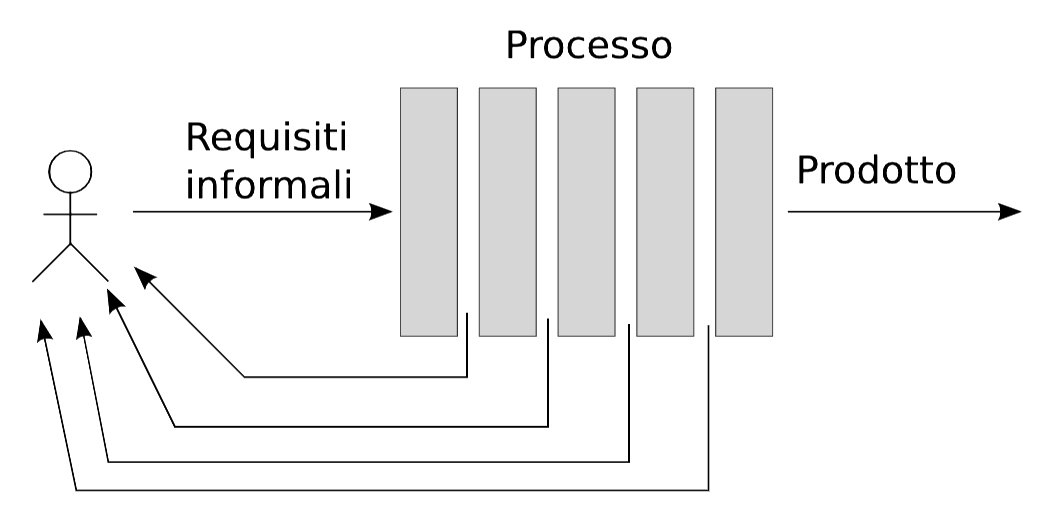
\includegraphics[width=0.8\linewidth]{assets/processo_esplicito.png}
    \caption{Se si segue un \textbf{modello esplicito} lo sviluppo software procede in modo ordinato e prevedibile (riduzione degli errori).}
\end{figure}

\begin{figure}[ht!]
    \centering
    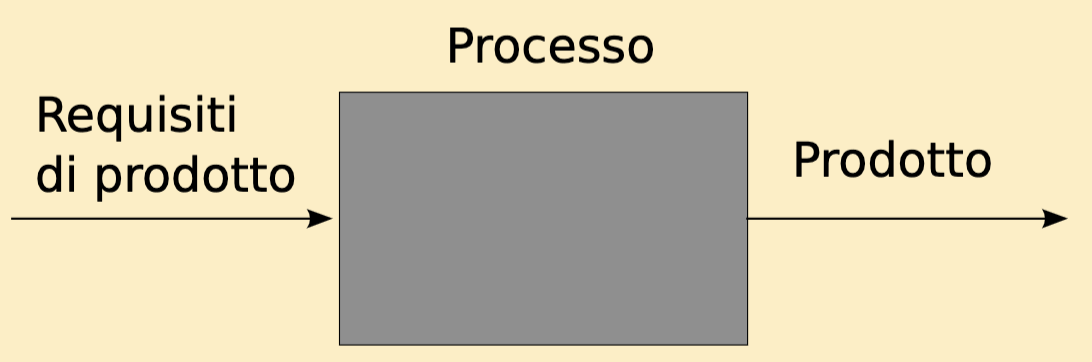
\includegraphics[width=0.8\linewidth]{assets/processo_blackbox.png}
    \caption{Se NON si segue un modello preciso lo sviluppo viene considerato una scatola nera (\textbf{black box}), in cui gli input sono i requisiti del prodotto e l'output il prodotto stesso.}
\end{figure}

\newpage

\section{Attività del processo di sviluppo}
Attività fondamentali del processo di produzione software. Devono essere eseguite a prescindere dal modello di sviluppo adottato. Ogni fase restituisce un \textit{artefatto} in output. Gli \textit{artefatti intermedi} (non rilasciati al cliente) contribuiscono al prodotto finale (sistema software).

\subsection{Studio di fattibilità}
Viene eseguito da personale qualificato, consiste in una simulazione del processo di sviluppo sotto vari scenari. Ha come output un documento che:
\begin{itemize}
    \item Definisce il problema
    \item Elenca soluzioni alternative (costi e benefici)
    \item Esplicita risorse richieste, costi e date di consegna
\end{itemize}
La \textit{\textbf{SWOT Analysis}} è uno strumento di pianificazione strategica per progetti che richiedono decisioni a ogni raggiungimento di obiettivo. Distingue i seguenti elementi:
\begin{itemize}
    \item \textit{Strengths}: interne al progetto, utili.
    \item \textit{Weaknesses}: interne al progetto, di ostacolo.
    \item \textit{Opportunities}: esterne al progetto, vantaggiose.
    \item \textit{Threats}: esterne al progetto, di impedimento.
\end{itemize}

\subsection{Analisi e specifica dei requisiti}
Consiste nel:
\begin{itemize}
    \item stabilire se le richieste del cliente (\textit{requisiti}) siano soddisfacibili e con quale grado di qualità;
    \item formalizzare le richieste in una serie di \textit{features} che l'applicazione deve assicurare (in un \textit{documento di specifica});
    \item occuparsi dell'individuazione degli \textit{stakeholder} (persone, aziende, entità interessate al sistema).
\end{itemize}

\paragraph{Modularizzazione orizzontale} Consiste nell'analizzare il progetto sullo stesso piano di astrazione da diversi punti di vista (uno per ogni aspetto del problema), strutturando il sistema come collezione di viste come:
\begin{itemize}
    \item \textit{Modello dei dati} (Diagramma ER, Class diagram)
    \item \textit{Modello delle funzioni eseguibili} (Flow o Use Case diagram)
    \item \textit{Modello di controllo di esecuzione} (Reti di Petri, State diagram)
\end{itemize}

\paragraph{Classificazione dei requisiti}
\begin{itemize}
    \item \textbf{MUST}: relativi alla \textit{correttezza}, requisiti minimi per considerare il sistema accettabile;
    \item \textbf{SHOULD}: relativi alla \textit{robustezza}, requisiti desiderabili, ma la cui omissione non compromette le funzionalità di base;
    \item \textbf{MAY}: requisiti facoltativi, tralasciabili in caso di mancanza di risorse.
\end{itemize}

\paragraph{Documento di specifica} Output di questa fase, sottoposto agli stakeholder. Deve essere comprensibile, preciso, completo, consistente, non ambiguo e facile da modificare. Può contenere un piano di test del sistema e/o una versione preliminare del manuale utente. È strutturato come segue:
\begin{itemize}
    \item \textit{Dominio}: breve descrizione del dominio applicativo e obiettivi da raggiungere.
    \item \textit{Requisiti funzionali}: descrivono cosa dovrà fare il prodotto (formali).
    \item \textit{Requisiti non funzionali}
    \item \textit{Requisiti del processo di sviluppo e manutenzione}: procedure di controllo qualità, priorità di sviluppo, possibili cambiamenti del sistema.
\end{itemize}

\subsection{Definizione e progettazione dell'architettura software}
Produzione di un \textit{documento di specifica di progetto} che descrive la struttura del sistema in termini di \textit{componenti}, relative interfacce e relazioni fra essi (motivando ogni scelta). Può richiedere l'uso di notazioni standard (come \textit{UML}).

\subsection{Produzione di codice e test di moduli}
Il team di programmatori procede a implementare e testare i singoli moduli (in maniera indipendente). L'output di questa fase è il codice sorgente dei moduli.

\subsection{Integrazione e test del sistema}
Fase di assemblaggio del sistema a partire dai singoli moduli (seguendo criteri \textit{top-down} o \textit{bottom-up}). Nel caso di modelli incrementali i moduli sono sviluppati, testati e integrati nel sistema man mano. L'applicazione completa viene sottoposta a un primo test (\textbf{\textit{"Alpha test"}}).

\subsection{Rilascio, installazione e manutenzione}
Il \textit{rilascio} avviene in due fasi:
\begin{itemize}
    \item Distribuzione a un gruppo selezionato di clienti (\textbf{\textit{"Beta test"}})
    \item Rilascio ufficiale sul mercato (\textit{\textbf{"Release"}})
\end{itemize}
L'\textit{installazione} definisce l'architettura del sistema a tempo di esecuzione.
La \textit{manutenzione} ha inizio (fase più costosa, 60\% c.d.p.):
\begin{itemize}
    \item Adattiva, correttiva (20\% c.d.m.)
    \item Perfettiva (50\% c.d.p.)
\end{itemize}

\newpage